\documentclass[11pt,a4paper]{jsarticle}
\usepackage[dvips]{graphicx}
\usepackage{fancyhdr}
\setcounter{page}{0}
%
\begin{document}

\title{制御工学実験II \\ 2.直流モータのモデリング}
\author{提出者 \\ 14104064 下松八重 宏太 \\ \\ 共同実験者 \\ 14101028 梶野 翔平 \\ 14104092 中島 美香 \\ 16104311 北山 拓夢 \\ 13104119 廣瀬 直人}
\date{提出日 \today}



\maketitle
\thispagestyle{empty}
\newpage


 \section{目的}
  直流モータ(DCモータ)は様々な工業製品に組み込まれており,制御工学で利用される基本的なアクチュエータの一つである.直流モータの自動制御に関する応用分野は広いため,直流モータを制御する技術を修得することは重要である.本実験の目的は,直流モータの種々のパラメータと直流モータが組み込まれたシステムの伝達関数の同定を行うことである.また,これらの作業を通じて制御系設計のためのモデリング技術を研くことも目的の一つである.
 \section{原理}
  本実験で扱う直流モータが組み込まれたシステムは直流モータとそれに付加された慣性負荷,パワーアンプ,ロータリエンコーダ,フィルタから構成される.このシステムの直流モータ周辺の電気的構成の概要とブロック線図を図\ref{block1}に示す.
 
 \begin{figure}[bp]
  \begin{center}
   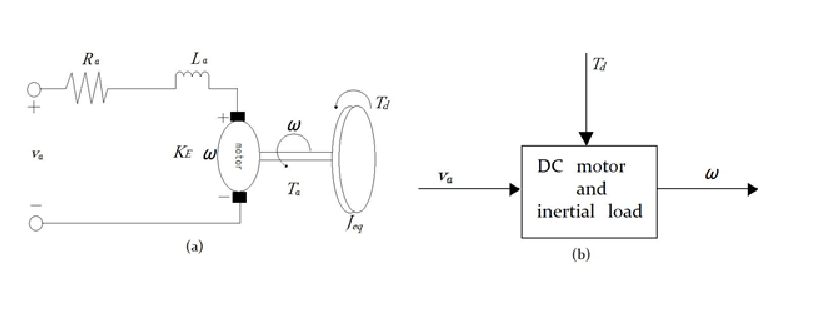
\includegraphics[scale = .8]{./picture/block1.eps}
   \caption{直流モータの(a)電気的構成図と(b)入出力関係}
   \label{block1}
  \end{center}
 \end{figure}
  \subsection{直流モータの力学的方程式の導出}
  まず,モータトルク定数と誘起電圧定数の関係を導出する.電機子に発生するトルクを{\it T}[Nm],電機子電流を{\it i}[A]とし,磁界の強さが一定であると仮定すれば,Bli則を用いて,
  \begin{equation}
   T = K_a \Phi i = K_T i
    \label{eq1}
  \end{equation}
  となる.ここで,$K_a$は設計パラメータであり,$\Phi$[Wb]は磁界の一磁極あたりに発生する磁束,$k_T$[N$\cdot$m/A]はトルク定数である.一方,モータロータ内の導線が外力によって角速度$\omega$[rad/s]で回転している時には,導線に以下の逆起電力が発生する.
  \begin{equation}
   T = K_a \phi_\omega = K_E \omega
    \label{eq2}
  \end{equation}
  ここで$K_E$[V$\cdot$s/rad]は誘起電圧定数であり,式\ref{eq1}と式\ref{eq2}の関係より$K_E$と$K_T$の値はSI単位系を用いる限り等しくなる.\\
  次に直流モータの電気的時定数を導出する.電気的時定数とは,モータ内を流れる電流の時間応答の早さを表す定数である.ある直流モータの回転軸を拘束して一定電圧を印加し,電流が定常値の63.2\%に到達するまでの時間で表される.キルヒホッフの法則より,一般的な直流モータを表す電気的関係式は
  \begin{equation}
   v_a (t) = R_a i_a (t) + L_a i_a (t) + K_E \omega (t)
    \label{eq3}
  \end{equation}
  と表せる.この式をラプラス変換すると
  \begin{equation}
   V_a (s) = R_a I_a (s) + sL_a I_a (s) + K_E \Omega (s)
    \label{eq4}\label{block1}
  \end{equation}
  となる.ここで,軸が固定された状態,すなわち$\Omega (s) = 0$とすると直流モータの印加電圧からモータ内部の電流への伝達関数は
  \begin{equation}
   G_{{i_a},{v_a}} (s) = \frac{I_a(s)}{V_a(s)} = \frac{1}{R_a + sL_a} = \frac{\frac{1}{R_a}}{1+s\frac{L_a}{R_a}}
    \label{eq5}
  \end{equation}
  となる.これよりモータの電気的時定数は
  \begin{equation}
   \tau_e  = \frac{L_a}{R_a}
    \label{eq6}
  \end{equation}
  であることがわかる.また,本実験で利用する直流モータの公称値は$L_a = 0.82$[mH],$R_a = 10.6$[$\Omega$]であるので,電気的時定数は
  \begin{equation}
   \tau_e = 0.0000774[s]
    \label{eq7}
  \end{equation}
  であり,以下に示す機械的時定数と比べて非常に小さい値である.したがってこの値は無視できると考えると,式\ref{eq4}を
  \begin{equation}
   V_a(s) \simeq R_a I_a(s) + K_E \Omega(s)
    \label{eq8}
  \end{equation}
  と簡略化出来る.\\
  直流モータの力学的方程式を導出する.まず,直流モータの軸摩擦を無視すると,運動方程式は以下のように表せる.
  \begin{equation}
   J_{eq} \dot{\omega}(t) = K_T i_a(t) + T_s(t) 
    \label{eq9}
  \end{equation}
  次に,この式をラプラス変換し,式\ref{eq8}より
  \begin{equation}
   (sJ_{eq} + \frac{K_T^2}{R_a})\Omega(s) = \frac{K_T}{R_a} V_a(s) + T_d(s)
    \label{eq10}
  \end{equation}
  を得る.これより,印加電圧からモータ軸の回転速度への伝達関数を得るために$T_s(s) = 0$として
  \begin{equation}
   G_{\omega , V_a}(s) = \frac{\Omega(s)}{V_a(s)} = \frac{K}{\tau s+1}
    \label{eq11}
  \end{equation}
  を得る.ただし,
  \begin{equation}
   K = \frac{1}{K_T} , \tau = \frac{J_{eq} R_a}{K_T^2}
    \label{eq12}
  \end{equation}
  である.$\tau$はモータの機械的時定数と呼ばれる.\\
  次に外乱トルク$T_d$からモータ軸の回転速度への伝達関数は式\ref{eq10}より,$V_a(s) = 0$として,
  \begin{eqnarray}
   G_{\omega , T_d}(s) = \frac{\Omega(s)}{T_d(s)} = \frac{K_{T_d}}{\tau_{T_d} s+1}
    \label{eq13}
  \end{eqnarray}
  である.
  \begin{figure}[hbp]
   \begin{center}
    \includegraphics[scale = .8]{./picture/block2.eps}
    \caption{直流モータシステムのブロック線図}
   \end{center}
  \end{figure}
  
  \newpage
  
 \section{実験方法}
  \subsection{モデリングモジュールプログラム}
  QICiiモデリングモジュールプログラムを利用して、実験機の直流モータのモデリングを行う。\\
  このプログラムでは、実際の直流モータの駆動と並行してシステムのシミュレーションも実行することができる。このシミュレーションの出力は、モデル化の結果の検証やモデルフィッティングに利用することができる。シミュレーションプログラムへの入力値は実際のモータへの入力電圧と等しく、シミュレーションの出力結果は赤色の実線、実際のモータ速度は青色の実線で同じウィンドウに表示される。このプログラムによりシミュレートされるモータ軸の回転速度$\omega_s$はモデル化された伝達関数と実際のモータへの印加電圧から以下のように計算される。
  \begin{equation}
   \omega_s(s) = \frac{KV_a(s)}{\tau s+1}
    \label{eq14}
  \end{equation}
  また,実験機のサンプル周期は$h = 0.01[s]$である.
  \subsection{電機子抵抗値の同定}
  以下の手順にしたがって電機子抵抗値の同定を行う.
  \begin{enumerate}
   \item 生成される信号振幅を0に設定する.
   \item 電圧0でのバイアス電流$I_{bias}$を測定する.
   \item モータ軸を動かないように手で保持する.
   \item Offsetに-5[V]から5[V]までの電圧を1[V]刻みで入力する.
   \item 各電圧に対する電流値を計測し,これからバイアス電流を減じて抵抗値を計算する.
  \end{enumerate}
  ただし,電流値がディスプレイに表示されるまで時間遅れがあるため,各電流の計測は表示される値が整定するまで待つ必要がする.
  \subsection{トルク定数及び誘起電圧定数の同定}
  以下の手順に従って誘起電圧定数を同定する.
  \begin{enumerate}
   \item 生成される信号振幅を0に設定する.
   \item 電圧0でのバイアス電流$I_{bias}$を測定する.
   \item モータ軸を動かないように手で保持する.
   \item Offsetに-5[V]から5[V]までの電圧を1[V]刻みで入力する.
   \item 各電圧に対する回転速度と電流値を計測し,電流値からバイアス電流を減ずる.
   \item 式\ref{eq8}より誘起電圧定数を同定する.
  \end{enumerate}
  式\ref{eq8}の計算には上で求めた抵抗値を利用する.
  \subsection{モデル検証をモデルフィッテイング}
  モデル化の精度を向上させるためのモデルフィッテイングを行う.
  \begin{enumerate}
   \item 入力を矩形波に設定し,振幅や周波数などを適切な値に設定する.
   \item 前の実験で求めたパラメータ$K$と$\tau$の値を入力し,実験をシミュレーションを開始する.
   \item 満足できる応答の一致が得られるまで,$K$と$\tau$の値を調整する.
  \end{enumerate}
 \section{結果}
  \subsection{電機子抵抗値の同定}
  測定結果を表\ref{table1}に示す.バイアス電流$I_{bias} = -0.027[A]$であった.
  \begin{table}[hbp]
   \begin{center}
    \caption{電機子抵抗値の同定結果}
     \begin{tabular}{|c|c|c|} \hline
      電圧[V] & 出力電流 - バイアス電流[A] & 電機子抵抗値[$\Omega$] \\ \hline \hline
      5.0 & 0.347 & 14.41 \\ \hline
      4.0 & 0.232 & 17.24 \\ \hline
      3.0 & 0.170 & 17.65 \\ \hline
      2.0 & 0.106 & 18.87 \\ \hline
      1.0 & 0.029 & 34.49 \\ \hline
      0.0 & 0.000 & - \\ \hline
      -1.0 & -0.027 & 37.04 \\ \hline
      -2.0 & -0.091 & 21.98 \\ \hline
      -3.0 & -0.157 & 19.11 \\ \hline
      -4.0 & -0.206 & 19.42 \\ \hline
      -5.0 & -0.306 & 16.34 \\ \hline
      - & 平均値$\bar{R_a}$ & 21.65 \\ \hline
     \end{tabular}
    \label{table1}
   \end{center}
  \end{table}

\newpage


  \subsection{誘起電圧定数の同定}
  測定結果を表\ref{table2}に示す.バイアス電流$I_{bias} = -0.027[A]$であった.\\
   \begin{table}[b]
    \begin{center}
     \caption{誘起電圧定数の同定結果}
     \begin{tabular}{|c|c|c|c|} \hline
      電圧[V] & 出力電流 - バイアス電流[A] & 回転速度[rad/s] & 誘起電圧定数 $K_E$ \\ \hline \hline
      5.0 & 0.007 & 92 & 0.0527 \\ \hline
      4.0 & 0.007 & 73 & 0.0527 \\ \hline
      3.0 & 0.007 & 54 & 0.0528 \\ \hline
      2.0 & 0.007 & 35 & 0.0528 \\ \hline
      1.0 & 0.007 & 16 & 0.0530 \\ \hline
      0.0 & 0.000 & 0 & - \\ \hline
      -1.0 & -0.007 & -17 & 0.0499 \\ \hline
      -2.0 & -0.007 & -35 & 0.0528 \\ \hline
      -3.0 & -0.007 & -54 & 0.0528 \\ \hline
      -4.0 & -0.007 & -73 & 0.0527 \\ \hline
      -5.0 & -0.007 & -92 & 0.0527 \\ \hline
      & & 平均値$\bar{K_E}$ & 0.0525 \\ \hline
     \end{tabular}
     \label{table2}
    \end{center}
   \end{table}
   このとき,シミュレーションパラメータ$K$と$\tau$は
   \begin{eqnarray}
    K = \frac{1}{K_E} = \frac{1}{0.0525} \simeq 19.05 \\
    \tau & = & \frac{J_{eq} R_a}{K_E^2} \nonumber \\
    & \simeq & 0.173
   \end{eqnarray}
   である.したがって,伝達関数は
   \begin{equation}
    G_{\omega , v_a}(s) = \frac{19.05}{0.0173s+1}
   \end{equation}
   となる.
  \subsection{モデル検証とモデルフィッテイング}
  検証によりシミュレーションパラメータ$K = 18.5$,時定数$\tau = 0.1$とした.
  実験値,公称値,モデルフィッテイングによるシミュレーション結果を図3,4,5に示す.

  \newpage

 \section{考察}
  \subsection{電機子抵抗値の誤差}
  実験で求めた抵抗値$\bar{R_a}$と公称値との相対誤差は$4.4\%$となった.\\
  これは電流値を測定するときに電流値がぶれていたために,電流値を正確に読み取れなかったためと考える.また,モータの回転軸を人の手で固定したために完全に固定することが出来ず,正確な電流値が測定できず誤差が生じたを考える.
  \subsection{伝達関数の比較}
  実験値,公称値,モデルフィッテイングによる伝達関数を比較する.図4において公称値によるシミュレーションの結果では角速度の誤差が生じている.逆に,実験値によるシミュレーションの結果では公称値によるものよりも誤差が小さい.これは理想的な伝達関数を求めた際,外乱による影響を考えずに導出したため公称値によるシミュレーション結果に誤差が生じたと考える.実験値による$K$と$\tau$は外乱の影響が含まれた値となっているため,誤差が小さくなったと考える. \\
  次に調整したパラメータと実験値との相対誤差を求めると
  \begin{eqnarray}
   \Delta K & = & \frac{19.05-18.5}{18.5} \simeq 0.0298 \\
   \Delta \tau & = & \frac{0.173-0.1}{0.1} \simeq 0.735 
  \end{eqnarray}
  となり,それぞれ3\%と74\%であった.$K$の誤差よりも$\tau$の誤差が非常に大きく,図3において立ち上がり時間について誤差が生じている.したがって,ゲイン$K$は角速度の値に,時定数$\tau$は立ち上がり時間に影響を与えていることがわかる.立ち上がり時間と整定時間は時定数に比例しする.つまり,時定数が小さいほど目標値に早く到達する.また,ゲインは周波数伝達関数の絶対値のことをいう.
  
 \section{課題}
  \subsection{負荷外乱と測定ノイズ}
  本実験において考えられる負荷外乱は外乱トルク$T_d$であると考える.式\ref{eq13},\ref{eq14}より
  \begin{eqnarray}
   K_{T_d} & = & \frac{R_a}{K_t^2} \simeq 7859 , \tau_{T_d} = \frac{J_{eq} Ra}{K_T^2} \simeq 0.085 \\
   G_{\omega , T_d} & = & \frac{7859}{0.085s+1}
  \end{eqnarray}
  となる.ゲインが実験値よりも非常に大きく,$T_d$の値が入力電圧$v_a$より小さくても結果に大きな影響を与えると考えられる.\\
  測定ノイズについて,本実験で用いたロータリエンコーダによるものが考えられる.ロータリエンコーダはその分解能によって測定できる最小値が決まる.この標本化誤差が測定ノイズになったと考えられる.
  
  \subsection{無視されたパラメータ}
  本実験で無視されたパラメータはモータ電機子インダクタンス$L_a$である.このパラメータを無視しなかった場合の伝達関数を考える.式\ref{eq4},\ref{eq10}より
  \begin{equation}
   (sJ_{eq} + \frac{K_E^2}{R_a + sL_a})\Omega(s) = \frac{K_E}{R_a + sL_a}V_a(s) + T_d(s)
  \end{equation}
  であり,印加電圧からモータ軸の回転速度への伝達関数を得るために$T_d = 0$とすると
  \begin{equation}
   G_{\omega , v_a}(s) = \frac{\Omega(s)}{V_a(s)} = \frac{\frac{1}{K_E}}{\frac{J_{eq} L_a}{K_E^2} s^2 + \frac{J_{eq} R_a}{K_E^2} s + 1} 
  \end{equation}
  となる.これは2次遅れ系の伝達関数である.よってモータ電機子インダクタンス$L_a$を無視しなかった場合,この装置は2次遅れ系のシステムである.実験では伝達関数を1次遅れ系としたが,実際には2次遅れ系であることがわかる.

\newpage
\thispagestyle{fancy}
\rhead{再1}
\cfoot{}

 \section{理論的な伝達関数}
  公称値を利用して理論的な伝達関数$G_{\omega , v_a}(s), G_{\omega , T_d}(s)$及び慣性モーメント$J_eq$を求める.\\
  慣性モーメント$J_eq$はモータロータの慣性モーメント$J_M$と慣性負荷の慣性モーメント$J_L$の和で表される.$J_M = 1.16E-6, J_L = \frac{1}{2} M_l r_l^2$より公称値$M_l = 0.068, r_l = 0.0248$を用いて
 \begin{eqnarray*}
  J_eq & = & J_M + J_L \\
       & = & J_M + \frac{M_l r_l^2}{2} \\
       & = & 1.16 * 10^-6 + \frac{0.068 * 0.0248^2}{2} \\
 \end{eqnarray*}
 となる.式\ref{eq11}, \ref{eq12}より,$K_T = 0.0502, R_a = 10.6$なので
 \begin{eqnarray*}
 K & = & \frac{1}{K_T} \\
   & \simeq & 19.92 \\
\tau & = & \frac{J_eq R_a}{K_T^2} \\
     & \simeq & 0.093
 \end{eqnarray*}
これより
\begin{equation}
 G_{\omega , v_a}(s) = \frac{19.92}{0.093s + 1}
\end{equation}
式\ref{eq13},\ref{eq14}より同様にして
\begin{eqnarray*}
K_{T_d} & \simeq & 4206 , \tau_{T_d} = 0.093 \\
 G_{\omega , T_d} & = & \frac{4206}{0.093s + 1}
\end{eqnarray*}
である.

\section{課題の補足}
外乱トルクからモータ軸の回転速度への伝達関数のゲインが印加電圧からの伝達関数のゲインよりかなり大きくなっている.これにより,外乱トルクから実験結果への影響としてはシミュレーション結果の角速度の値に大きく影響していると考えられる.

\newpage
\thispagestyle{fancy}
\rhead{再々1}
\cfoot{}

\setcounter{section}{7}
\section{課題の補足}
測定ノイズについて,直流モータではブラシと電機子の接点で生じる.また,電機子の形状によって電機子電流が時間的変動を生じれば,トルクの時間的脈動につながる.直流モータには永久磁石を使われることが多いが,運転時に内部で生じる損失によって温度が上昇し,永久磁石の発生磁束がわずかに減少する.その他の測定ノイズとしては電源ケーブルやパソコンの画面などによる電気的ノイズ,シャフトのがたなどによる機械的ノイズなどが挙げられる.


\begin{thebibliography}{1}
 \bibitem{1}坂本哲三,``電気機器の電気力学と制御'',森北出版株式会社,2007,pp.161-164.
\end{thebibliography}


\end{document}









